\documentclass{beamer}

% --- THEME AND STYLING ---
\usetheme{Madrid} % A clean, professional theme with sections in the header.
\usecolortheme{default}
\setbeamertemplate{navigation symbols}{} % Hides navigation buttons
\setbeamertemplate{footline}[frame number] % Shows frame number in the footer

% --- PACKAGES ---
\usepackage[utf8]{inputenc}
\usepackage{graphicx} % To include images
\usepackage{hyperref} % For clickable links (good practice)
\usepackage{booktabs} % For better tables if needed

% --- PRESENTATION METADATA ---
\title[Project Satori]{Project Satori: AI Career Advisor}
\subtitle{Guiding India's Future, One Career at a Time}
\author{Omm Satyakam}
\institute{Team Satori}
\date{\today}

% --- DOCUMENT START ---
\begin{document}

% --- TITLE PAGE ---
\begin{frame}
  \titlepage
\end{frame}

% --- THE CHALLENGE ---
\begin{frame}
  \frametitle{The Challenge: Navigating the Career Maze}
  \begin{block}{The Problem}
    For millions of students across India, choosing a career path feels like standing at a daunting crossroads with a thousand branching paths and no map. They are inundated with generic advice but starved for guidance that speaks to their unique skills and dreams.
  \end{block}
  \begin{alertblock}{The Consequence}
    This leads to decision paralysis, missed opportunities, and a generation of talent struggling to find their place. Students need a trusted co-pilot for their career journey.
  \end{alertblock}
\end{frame}

% --- OUR SOLUTION ---
\begin{frame}
  \frametitle{Our Solution: Meet Satori ��}
  \textbf{Project Satori} is an intelligent, full-stack career advisor built to replace confusion with clarity. We provide a seamless, end-to-end platform that empowers students to discover, plan, and pursue their ideal careers with confidence.
  \vspace{0.5cm}
  \begin{enumerate}
  \item \textbf{Discover Your Path}: Our \textbf{Career Compass} assessment goes beyond surface-level questions to understand the user's core identity.
  \item \textbf{See Your Future}: The AI, powered by \textbf{LangChain + Gemini Pro}, generates \textbf{personalized career recommendations}.
  \item \textbf{Build Your Dream}: Satori then crafts a \textbf{detailed, week-by-week learning roadmap}.
  \item \textbf{Never Walk Alone}: Our \textbf{conversational AI Mentor} is available 24/7 for context-aware guidance.
  \end{enumerate}
\end{frame}

% --- WHAT MAKES SATORI UNIQUE? ---
\begin{frame}
  \frametitle{What Makes Satori Unique? ��}
  \begin{description}
    \item[End-to-End Platform] While other resources are fragmented, Satori unifies the entire process: discovery, planning, and mentorship are all in one place.
    \vspace{0.5cm}
    \item[A Mentor That Remembers] Our stateful AI Mentor understands context and remembers past conversations, providing continuous, interactive support.
    \vspace{0.5cm}
    \item[Intelligence with Purpose] We use distinct AI agents for recommendations, roadmaps, and mentorship, ensuring nuanced and accurate guidance.
  \end{description}
\end{frame}

% --- CORE FEATURES ---
\begin{frame}
  \frametitle{Core Features}
  \begin{itemize}
    \item �� \textbf{Secure JWT Authentication}: For a safe and personalized user experience.
    \item �� \textbf{Career Compass Questionnaire}: An interactive deep dive into a user's potential.
    \item �� \textbf{AI-Powered Recommendations}: Not just jobs, but tailored career callings.
    \item ��️ \textbf{AI-Generated Learning Roadmaps}: A step-by-step, actionable blueprint.
    \item �� \textbf{Stateful Mentor Chat}: An always-on AI companion for continuous guidance.
    \item ✨ \textbf{Modern UI/UX}: A beautiful, responsive interface (React + Tailwind).
    \item ⚙️ \textbf{Unified API Schema}: A robust and predictable backend.
  \end{itemize}
\end{frame}

% --- THE SATORI JOURNEY ---
\begin{frame}
  \frametitle{The Satori Journey: A User's Path to Purpose}
  \begin{figure}
    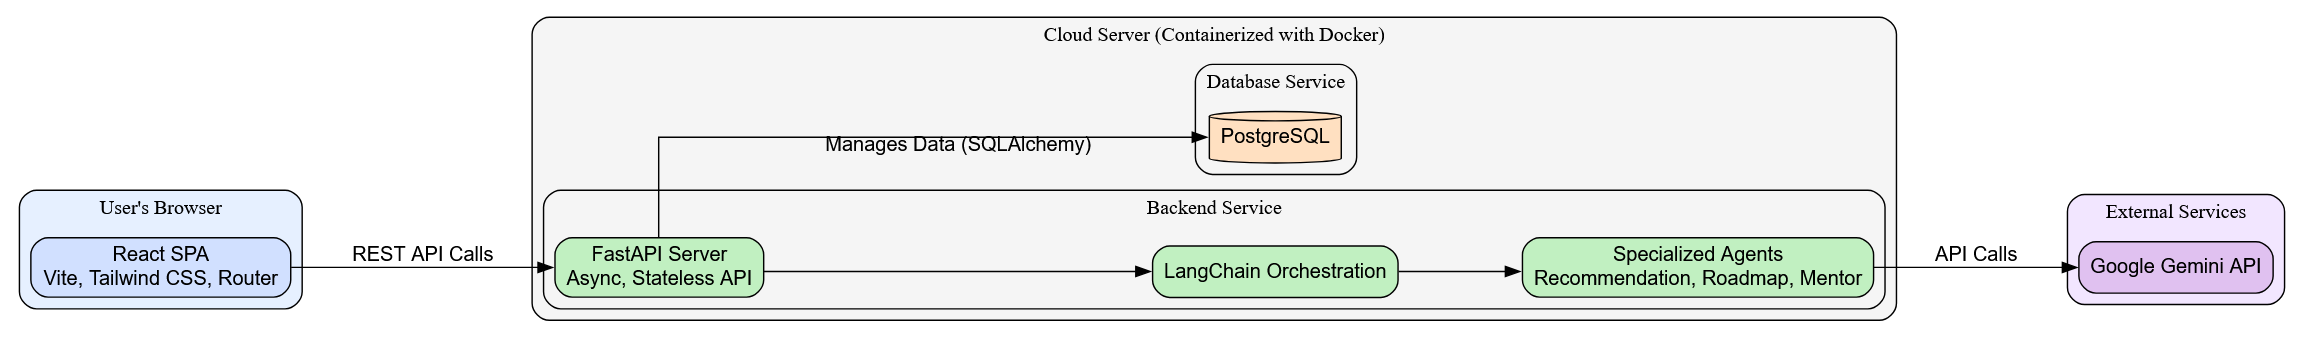
\includegraphics[width=\textwidth]{assets/user_flow_diagram.png}
    \caption{The Satori user journey, from sign-up to ongoing mentorship.}
  \end{figure}
\end{frame}

% --- OUR ARCHITECTURE ---
\begin{frame}
  \frametitle{Our Architecture: Built for Scale and Performance ��️}
    \begin{figure}
    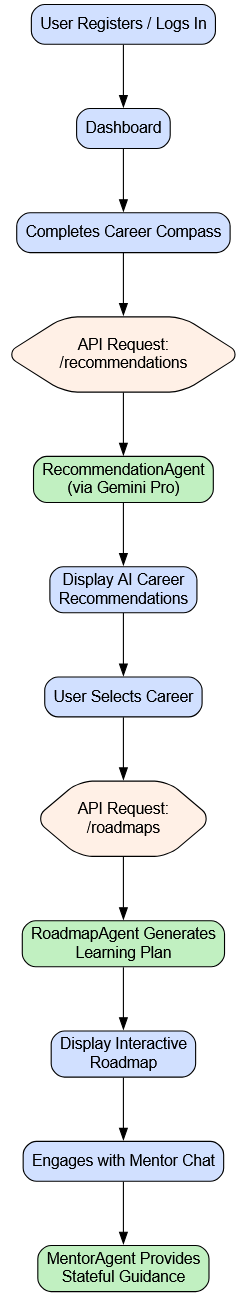
\includegraphics[height=0.8\textheight, keepaspectratio]{assets/architecture_diagram.png}
    \caption{Our high-level system architecture.}
  \end{figure}
\end{frame}

% --- THE TECH STACK ---
\begin{frame}
  \frametitle{The Tech Stack}
  \begin{columns}[T] % Two columns layout
    \begin{column}{0.5\textwidth}
      \begin{block}{Frontend}
        \begin{itemize}
          \item React \& Vite
          \item Tailwind CSS
          \item react-router-dom
        \end{itemize}
      \end{block}
      \begin{block}{AI}
        \begin{itemize}
          \item LangChain
          \item Google Gemini Pro \\ (\texttt{gemini-2.5-flash})
        \end{itemize}
      \end{block}
    \end{column}
    \begin{column}{0.5\textwidth}
      \begin{block}{Backend}
        \begin{itemize}
          \item Python \& FastAPI
          \item SQLAlchemy 2.0 (async)
        \end{itemize}
      \end{block}
      \begin{block}{Database \& DevOps}
        \begin{itemize}
          \item PostgreSQL
          \item Docker \& Docker Compose
          \item Poetry
        \end{itemize}
      \end{block}
    \end{column}
  \end{columns}
\end{frame}

% --- BUSINESS VIABILITY ---
\begin{frame}
  \frametitle{Business Viability: Lean, Scalable, \& Cost-Effective ��}
  Our architecture is not just powerful—it's incredibly efficient.
  \begin{itemize}
    \item \textbf{Lean Infrastructure}: The entire MVP runs seamlessly in a containerized environment on a single, low-cost VM.
    \item \textbf{Elastic Costs}: Our primary operational expense is the Gemini API, a pay-as-you-go service. Costs scale directly with user engagement.
    \item \textbf{MVP Ready}: With development complete, we have a market-ready product with minimal initial overhead.
  \end{itemize}
\end{frame}

% --- FINAL "THANK YOU" SLIDE ---
\begin{frame}
  \centering
  \vspace*{2cm}
  {\Huge Thank You}
  \vspace{1cm}
  
  {\large Project Satori}
\end{frame}

\end{document}